\section*{5. \"Ubung (Abgabe: 02.06.2010, 8.30 Uhr, schriftlich)}

\subsection*{1. Leiten Sie die Fouriertransformierte der Funktion $\delta_{x}(x,y):=\delta(x)$ her, wobei $\delta(x)$ die eindimensionale Dirac-Sto{\ss}-Funktion bezeichnet.}
%Siehe Abbildung \ref{fig:5.1}.
\begin{figure}[h] %  figure placement: here, top, bottom, or page
   \centering
   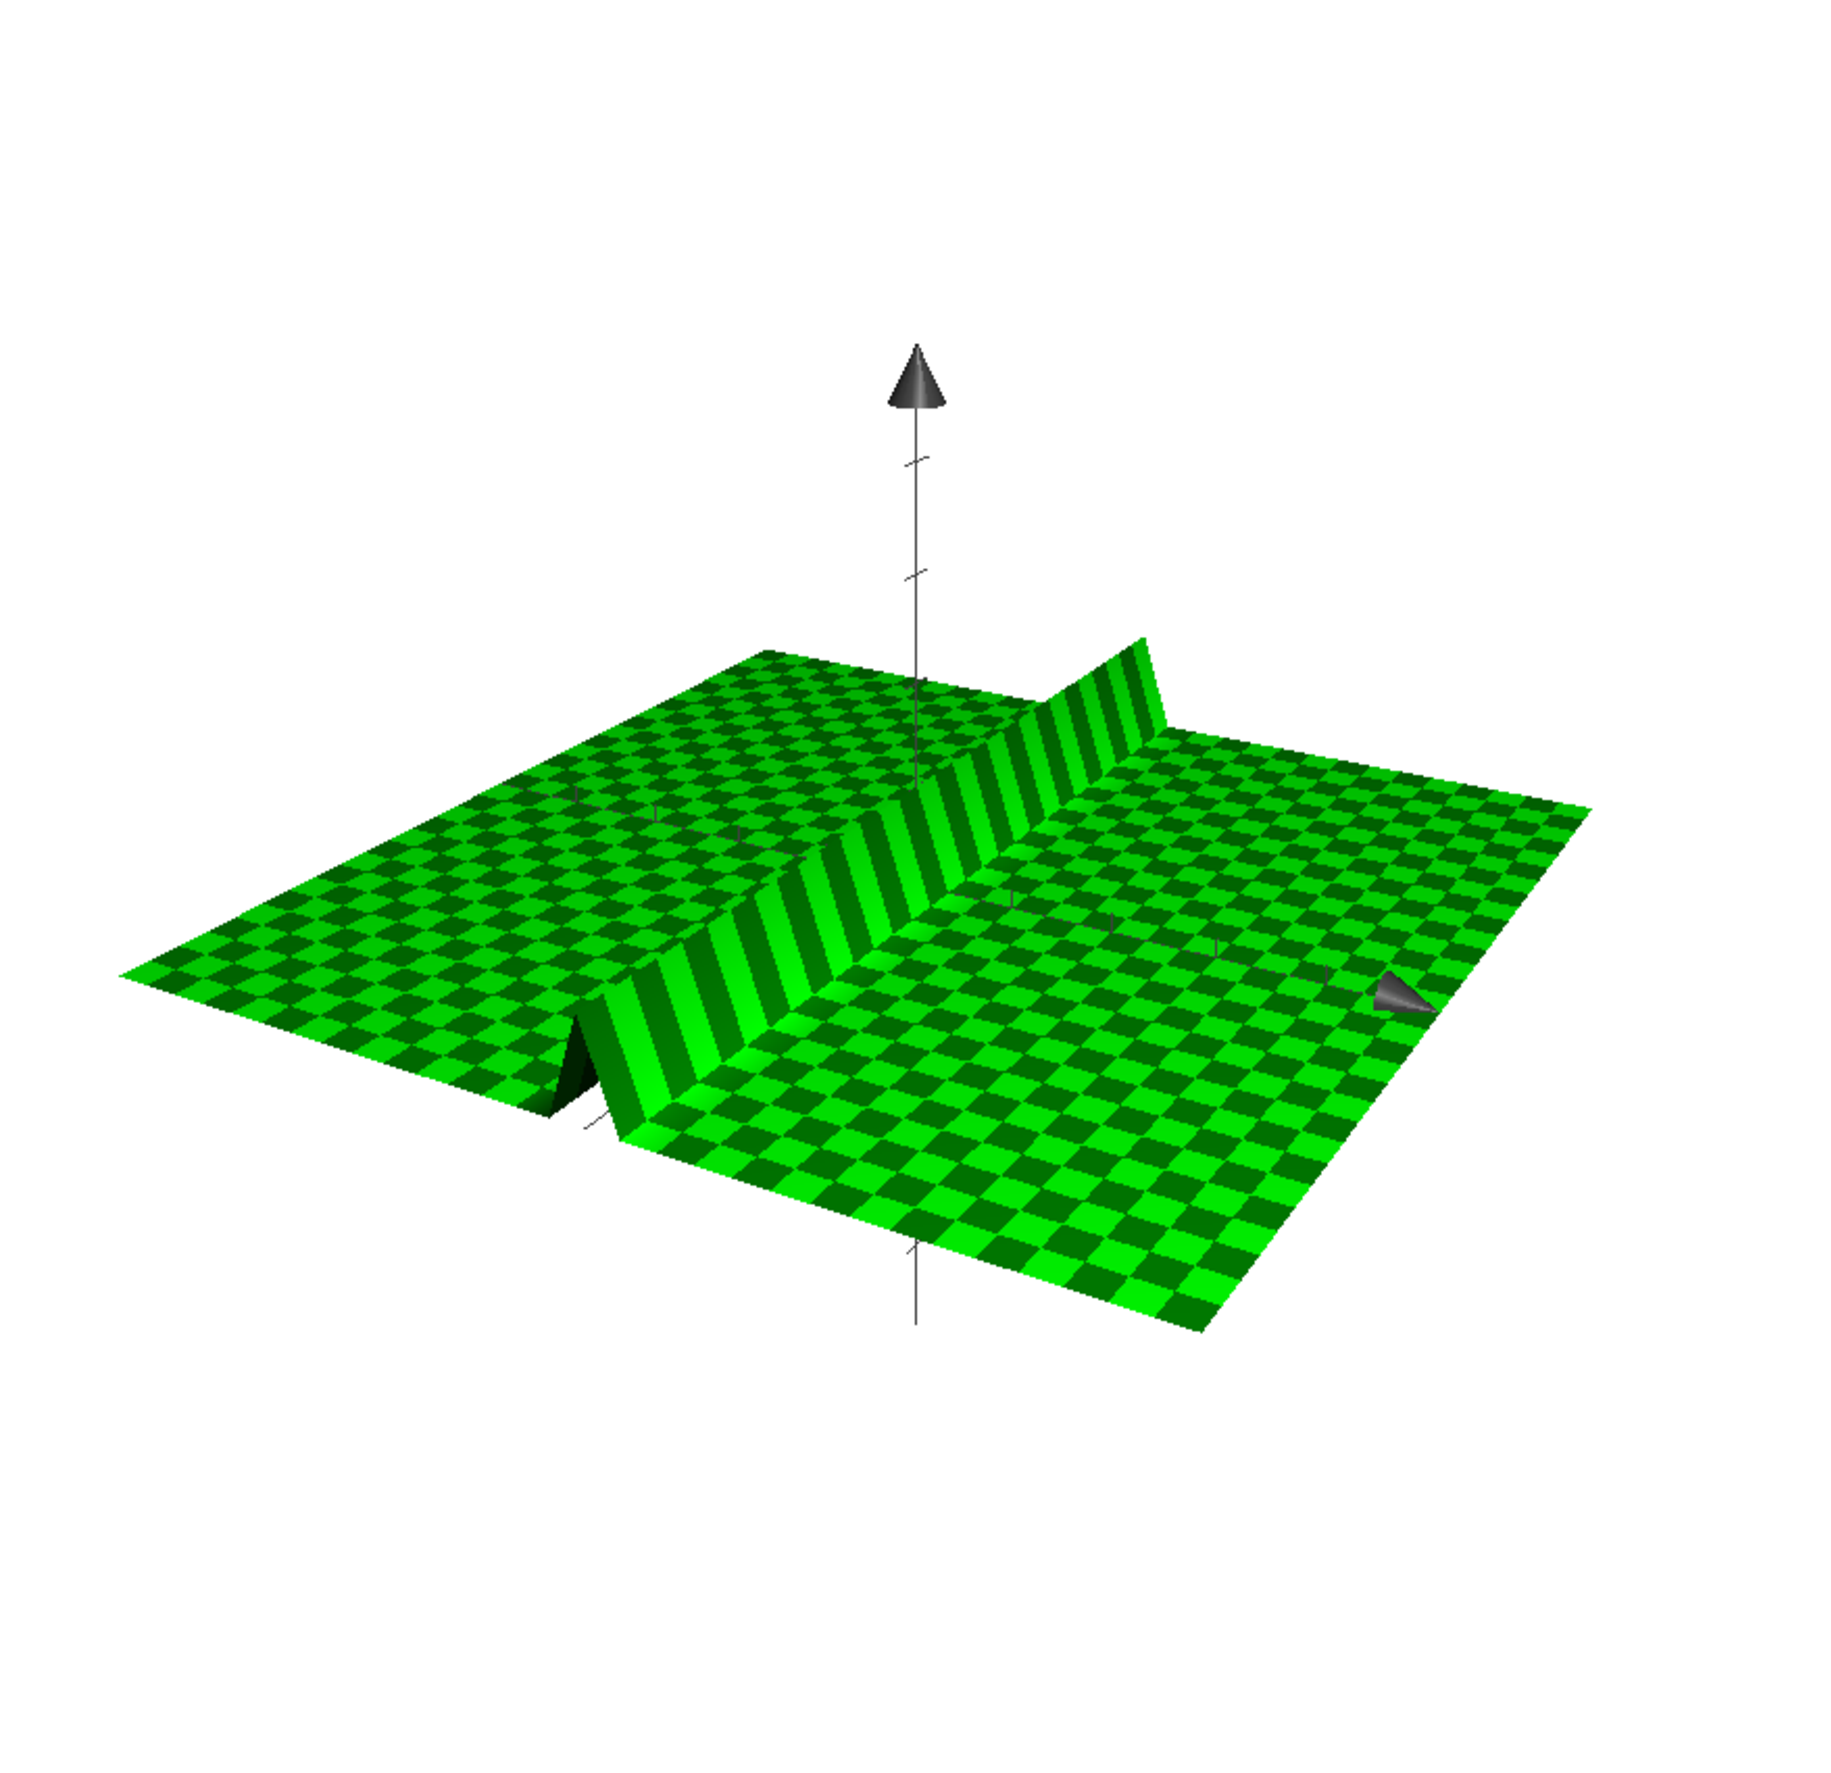
\includegraphics[width=0.8\textwidth]{Uebung5/5_1.pdf} 
   \caption{$\delta_{x}(x,y)$}
   \label{fig:5.1}
\end{figure}

\begin{eqnarray*}
f(x,y) & = & f_{x}(x)\cdot f_{y}(y) \\
\delta_{xy}(x,y) & = & \delta(x)\cdot\delta(y) \\
\delta_{x}(x,y) &=& \delta(x)\cdot 1(y) \\ \\
F(\delta(x)) &=& 1(\omega) \\ \\
F(\delta(x)\cdot 1(y)) &=& \delta(x) * 1(y) = 1(\omega) \; _{\square}
\end{eqnarray*}

\subsection*{2. Beschreiben Sie anschaulich das Ergebnis der Faltung eines zweidimensionalen Signals mit der Funktion $\delta_{x}(x,y)$. Was bedeutet dies im Frequenzbereich?}

\begin{eqnarray*}
\delta_{x}(x,y)*f(u,v) &=& \mathbf{F(\delta_{x}(x,y))}\cdot F(f(u,v)) \; \hbox{(Faltungstheorem)} \\
F(\delta_{x}(x,y)) &=& \mathbf{1(\omega)} \\
\end{eqnarray*}
\\
Im Ortsraum bedeutet die Faltung eine Ausblendung der x-Achse der zweidimensionalen Funktion. Die y-Achse bleibt erhalten (siehe Abbildung \ref{fig:5.1}). Dieses Ergebnis beruht auf der Sieb/Ausblend-Eigenschaft der $\delta$-Funktion. \\
Im Frequenzbereich bedeutet die Multiplikation mit $1(\omega)$ eine die zweidimensionale Funktion erhaltende (neutrale) Operation.

\subsection*{3. Berechnen Sie das Integral unter der Funktion $\delta^{2}(x,y):=\delta_{x}(x,y)\cdot\delta_{y}(y,x)$.}
\begin{align*}
& \int{\delta^{2}(x,y)~dx~dy}\\
= & \int{\delta_{x}(x,y)\cdot\delta_{y}(y,x)~dx~dy}\\
= & \int{\delta_{x}(x,y)~dx}~\cdot~\int{\delta_{y}(y,x)~dy}\\
= & \int{\delta(x) \cdot 1(y)~dx}~\cdot~\int{\delta(y) \cdot 1(x)~dy}\\
= & 1 \cdot 1\\
= & 1
\end{align*}

\subsection*{4. Gegeben sei eine beliebige reellwertige Bildfunktion $f(x,y)$. Nun faltet man diese Funktion mit einer geraden reellwertigen Funktion $g$ (d.h. $g(x,y)=g(-x,-y)$). Wie ver\"andert sich das Quadrat des Phasenspektrums?}
Phasenspektrum ist definiert als $\Phi = \arctan{\frac{Im(u,v)}{Re(u,v)}}$
Bei der Faltung einer beliebigen reellwertige Bildfunktion $f(x,y)$ mit einer geraden reellwertigen Funktion $g$ m\"ussen zwei F\"alle betrachtet werden:
\begin{enumerate}
\item Eine gerade reellwertige Bildfunktion $f(x,y)$ gefaltet mit $g$. Bei der Faltung entsteht wieder eine gerade reellwertige Funktion. Die Funktion besitzt nur einen reellen Anteil und keinen imagin\"aren. Daraus folgt f\"ur $\Phi^2$:\\
\begin{align*}
\Phi^2 &= (\arctan{\frac{0}{Re(u,v)}})^2\\
&= (\arctan(0))^2\\
&= 0
\end{align*}
\item Eine ungerade reellwertige Bildfunktion $f(x,y)$ gefaltet mit $g$. Bei der Faltung entsteht eine gerade reellwertige Funktion mit einem ungeraden Imagin\"aranteil. F\"ur das Phasenspektrum folgt:\\
\begin{align*}
\Phi^2 &= (\arctan{\frac{Im(u,v)}{Re(u,v)}})^2\\
&= \lim_{\frac{Im(u,v)}{Re(u,v)} \rightarrow \pm\infty} (\arctan{\frac{Im(u,v)}{Re(u,v)}})^2\\
&= \frac{\pi^2}{4}
\end{align*}
\end{enumerate}